\documentclass[border=4pt]{standalone}
\usepackage{tikz}
\usetikzlibrary{decorations.pathmorphing,arrows.meta}
\begin{document}
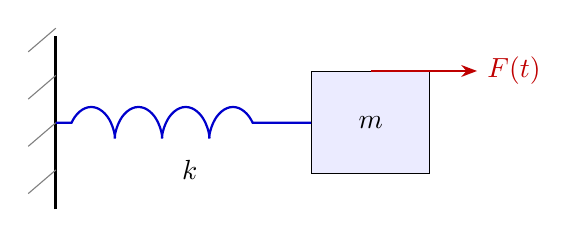
\begin{tikzpicture}
  \draw[line width=1pt] (0,-1.1) -- (0,1.1);
  \draw[gray] (-.35,-.9)--(0,-.6) (-.35,-.3)--(0,0) (-.35,.3)--(0,.6) (-.35,.9)--(0,1.2);
  \node[draw,fill=blue!8,minimum width=15mm,minimum height=13mm] (mass) at (4,0) {$m$};
  \draw[blue!80!black,line width=.8pt,decorate,
    decoration={coil,aspect=.5,segment length=6mm,amplitude=2mm,pre length=2mm,post length=2mm}]
    (0,0) -- (mass.west);
  \draw[-{Stealth[length=2mm]},red!75!black,line width=.8pt]
    (mass.north) -- ++(1.35,0) node[right] {$F(t)$};
  \node[below] at (1.7,-.35) {$k$};
\end{tikzpicture}
\end{document}
